\documentclass{scrartcl}
\usepackage[utf8]{inputenc}
\usepackage[english]{babel} % Trennung nach der neuen deutschen Rechtschreibung
\usepackage[utf8]{inputenc}
\usepackage[T1]{fontenc}
\usepackage{lmodern}

\usepackage{amsmath} % Erweiterte Mathematik-Umgebung
\usepackage{amsfonts} % zusätzliche Mathematik-Schrifttypen (v.a. \mathbb für Mengen)
\usepackage{ulem}

\usepackage{graphics}%soll beim Graphiken einfügen hilfreich sein
\usepackage{graphicx}
\usepackage{wrapfig}%lässt Textumflossene Bildeinbindung zu
\usepackage{epstopdf}%soll eps in pdf umwandeln


\titlehead{\centering University of Luxemburg}
\subject{Travaux Pratiques}
\title{Gyroscope}
\subtitle{J. Baller \\ M. Filimon}
\date{TP Session 08/10/2021}
\author{Louis-Hendrik Barboutie \\ Frederik Ehl \\ Florence Schmerber}

\begin{document}

\maketitle

\clearpage

\tableofcontents
	
\clearpage

\section{Introduction}

The aim of this experiment is to understand the principle of the gyroscope and to measure the moment of inertia as well as the angular speed of precession. The moment of inertia can be defined as the tendency of a rigid body to resist to angular acceleration. It is also known as rotational inertia. For measuring the moment of inertia we will be using the following equation: 

\begin{equation}
	\ I = \frac{grm-Mf}{ \alpha}
	\label{eq1}
\end{equation}

With $m$ being the mass applied on to the pulley, $g$ the gravity of earth, $r$ the radius of the disk, $\alpha$ the angular acceleration and $Mf$ being the frictional torque. 
\newline

Precession occurs when the orientation of the rotational axis of a rotation body is altered. It's the change of the first Euler angle.
Therefore we will be using this equation:

\begin{equation}
	\Omega = \frac{mgd}{I \omega}
	\label{eq2}
\end{equation}

$m$ is the mass of the rotating body, $g$ is, as said previously, the gravity of earth with the value $g=9.81 m/s^{2}$. $d$ is the distance between the center of the gyroscope axle, where it is attached to the bar, and the additional mass.Finally, $I$ is the moment of inertia of the rotating body and $\omega$ is the angular velocity of the rotating body.
\newline

We divided the experiment into two parts, first we measure the moment of Inertia $I$, then the angular speed of precession and discuss our observations.

\section{Experimental setup}
The setup we will be using is a simplified gyroscope. It is a solid disk rotating around the gyroscope axle, which is itself attached to a bar. To calibrate the gyroscope, two counterweights are attached at one end of the gyroscope axle. A pulley with an additional mass can be attached at the other end of the axle, near the disk, in order to actuate the disk.

\subsection{Determination of the moment of inertia}
To determine the moment of inertia, the gyroscope axle is fixed at the bar, which means it can't move either in the y or z axis. Then we wrap a string around the pulley with different masses between $25g$ to $125g$ and let the masses fall in order to act as a torque. We then measure the time the gyroscope takes for 4 revolutions. 

\subsection{Determination of the angular speed of precession}
On the other hand, in order to determine the angular speed of precession, the axle isn't fixed onto the bar so that the gyroscope can move freely. We add an additional mass of $153,18g$. We let the gyroscope rotate at a certain angular veocity $omega$ and measure the period of precession $T_{\Omega}$. In order to calculate the angular speed of precession we use the relation:
\begin{equation}
	\Omega = \frac{2\pi}{T_{\Omega}}
	\label{eq3}
\end{equation}

\section{Results}

\subsection{Determination of the moment of inertia}

    Under the assumption that $I \gg mr^2$, following linear relationship holds:
    
    \begin{equation}
        \alpha (m) = \frac{gr}{I} m - \frac{M_f}{I}
    \end{equation}
    
    Since all those terms are held constant, alpha is constant. We can then express the angle of rotation as a dependence of time as:
    
    \begin{equation}
        \phi(t) = \frac{1}{2} \alpha t^2
    \end{equation}

    Using our data (see appendix for individual analysis), for the time over four rotations, to plot $\phi(t)$, we can identify
    $\frac{1}{2} \alpha$ as the coefficient of the quadratic term of the trend line. This process was repeated for each mass separately. See appendix for the data tables. We obtain $\alpha(m)$ which we plot again, for which we obtain a linear trend line, for which the leading coefficient is (as in eq.(4)). By solving for I and plugging in our values we get:
    
    \begin{equation}
        \boxed {I \approx 1.24 \cdot 10^{-2} kg \cdot m^2}
    \end{equation}    
    
    We check if our assumption for eq.(4) is correct:
    
    \medskip
    
    \centering
    \begin{tabular}{|c|c|}
        \hline
        $m_i$ & $mr^2 (kg \cdot m^2)$ \\
        \hline
        $m_1$ & $2.1 \cdot 10^{-5}$ \\
        $m_2$ & $4.3 \cdot 10^{-5}$ \\
        $m_3$ & $6.4 \cdot 10^{-5}$ \\
        $m_4$ & $8.5 \cdot 10^{-5}$ \\
        $m_5$ & $1.1 \cdot 10^{-4}$ \\
        \hline
    \end{tabular}

    
    \flushleft
    
    \medskip
    
    For all of these values, the relation $I \gg mr^2$ holds.
    
    \medskip
    
    From eq.(4) and our data we can also determine the torque resulting from friction forces:
    \begin{equation}
        \boxed{M_f \approx -1.7 \cdot 10^{-3} kg \cdot m^2}
    \end{equation}
    
    
    
    \begin{figure}
        \centering
        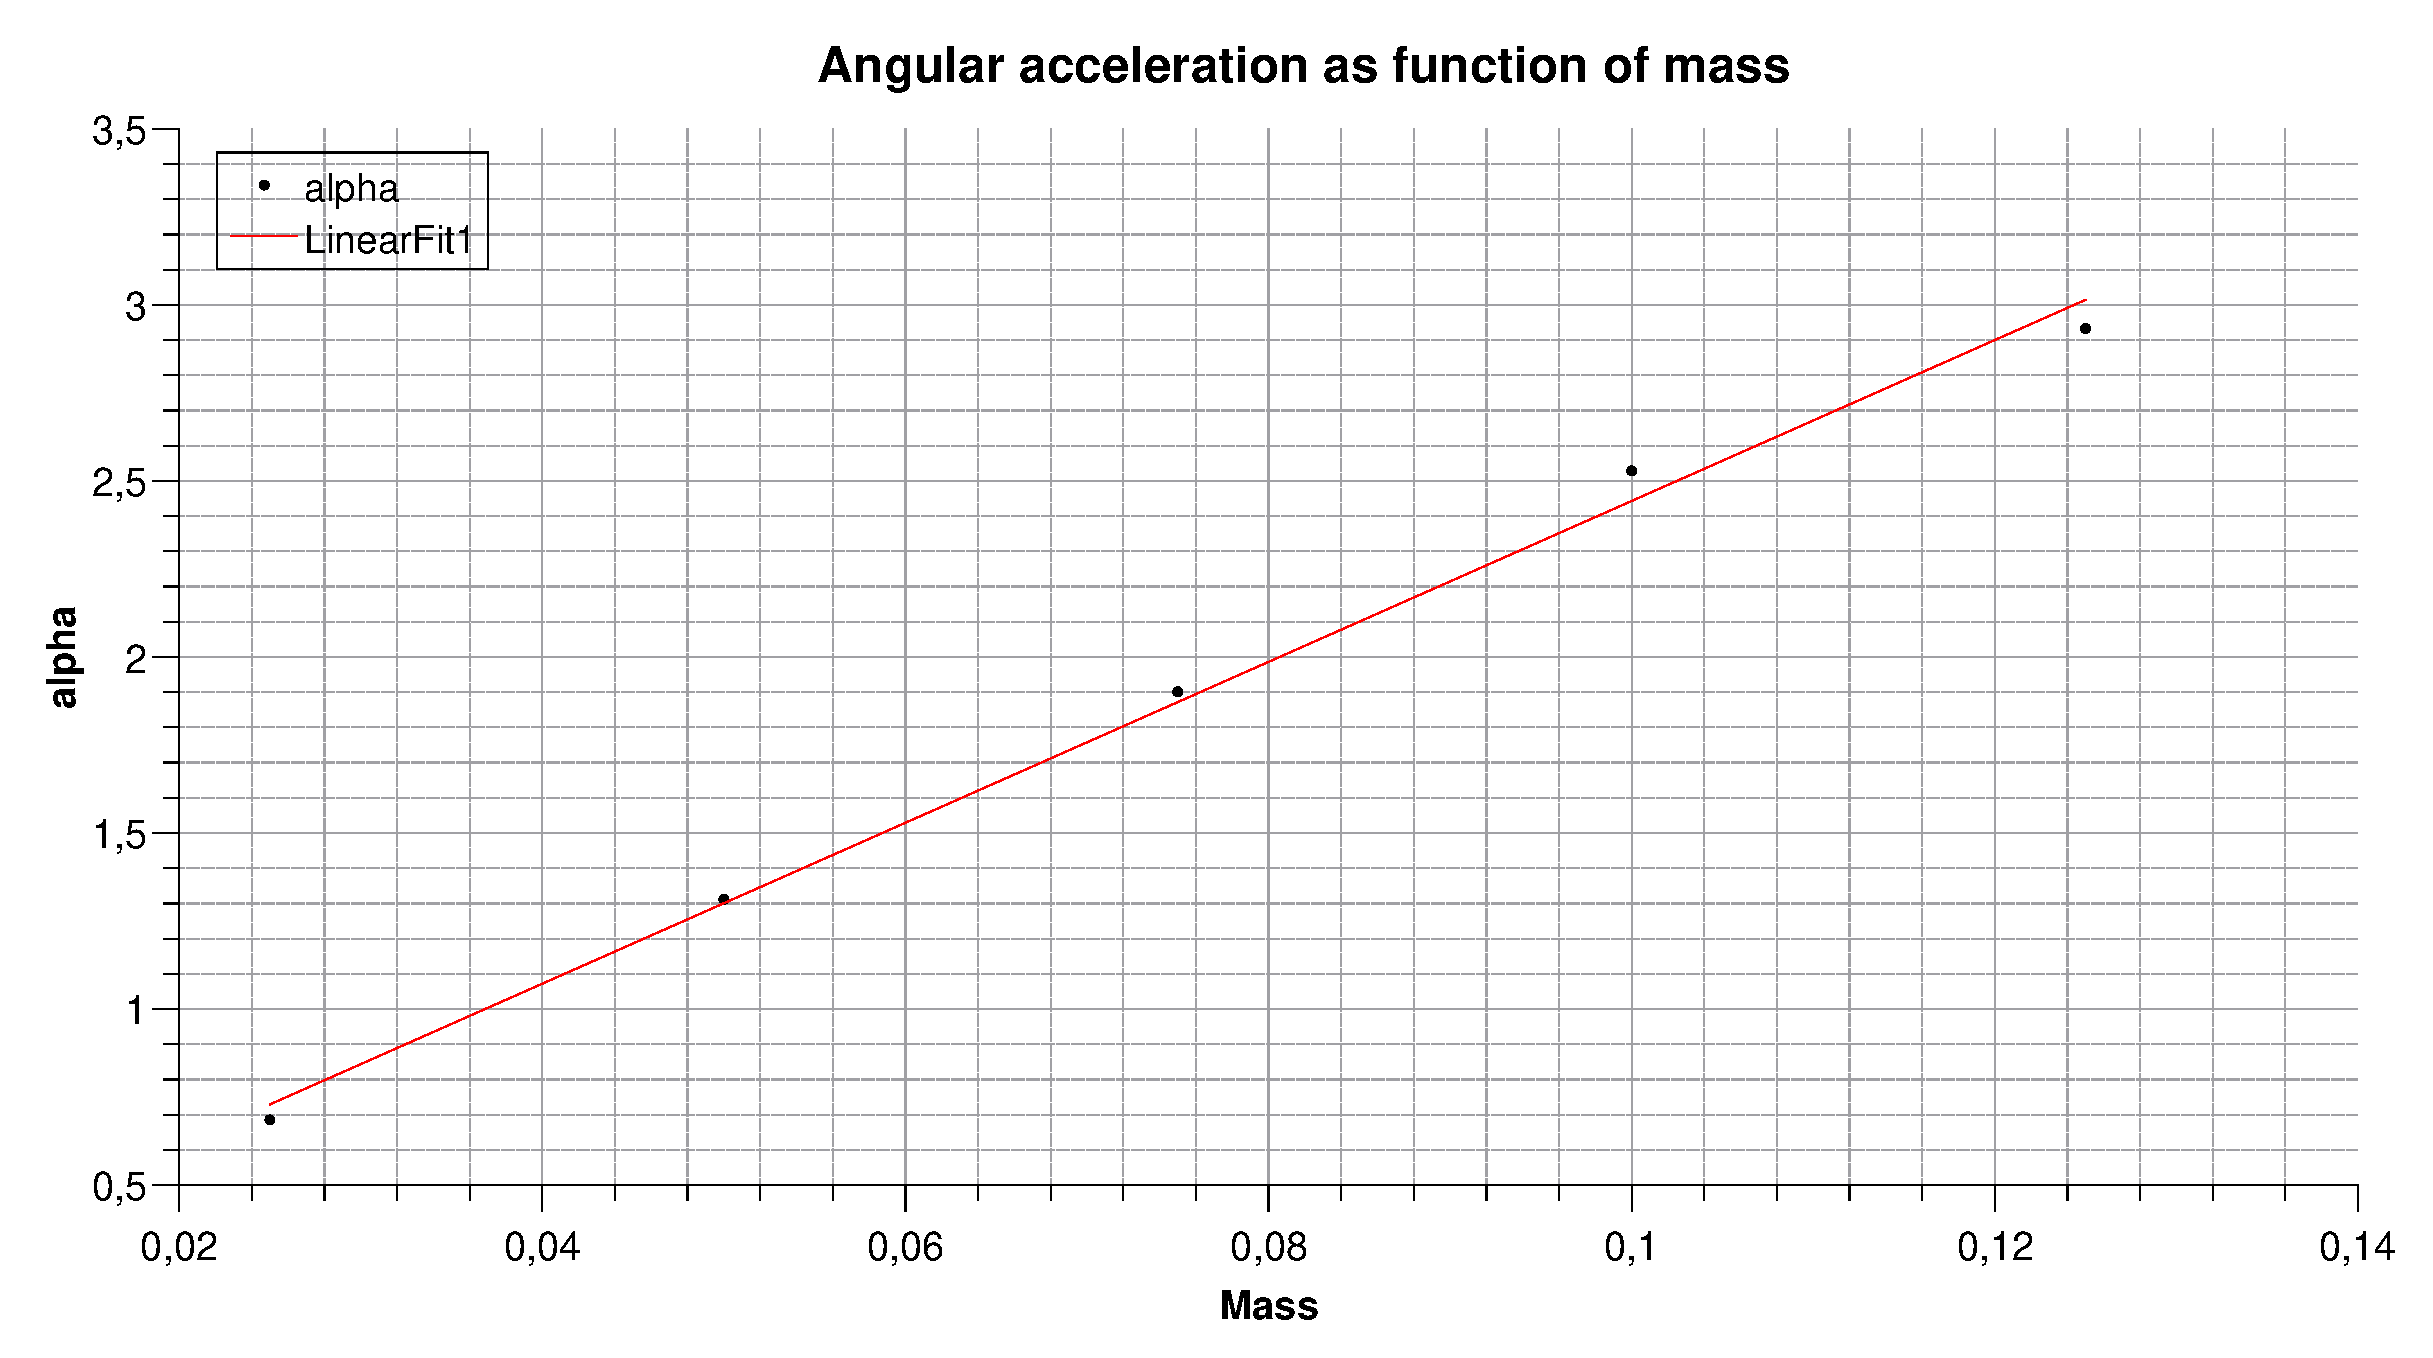
\includegraphics[width=14cm]{AlphaFunctionOfMass.eps}
        \caption{Caption}
        \label{fig:my_label}
    \end{figure}


\subsection{Determination of the speed of precession}
 First of all we need to equilibrate the gyroscope without extra added weight, so that $\sum \vec{f} = \vec{0}$.
 Next we apply an extra weight at the front of the axis, which leads to a constant gravitational force. Once the disc is actuated it's angular momentum and the torque applied to the axis of the gyroscope lead to a rotation of the gyroscope around the vertical axis. This phenomenon is called precession, where the angular momentum vector of the rotating disc chases the vector of the torque applied to the axis.
 In order to determine the angular velocity of precession $\Omega$ we first measure the angular velocity of the gyroscope $\omega$ using the provided RPM-measuring device. With a stopwatch we identify the precession period T. We then measure $\omega$ again, so we can take the average of both values in order to minimize the effect of friction. Using the relation 
 \begin{equation}
     \Omega = \frac{2\pi}{T}
 \end{equation}
 we calculate the experimental value of the angular speed of precession.
 
 \medskip
 \centering
 \begin{tabular}{|c|c|c|c|c|}
    \hline
    $rpm_1$ & $rpm_2$ & $\omega_1$ & $\omega_2$ & $\bar{\omega}$ \\
    \hline
    $364$ & $346$ & $38,11$ & $36,23$ & $37,18$ \\
    \hline
    $336$ & $324$ & $35,19$ & $33,93$ & $34,56$ \\
    \hline
    $330$ & $318$ & $34,56$ & $33,30$ & $33,93$ \\
    \hline
    $307$ & $303$ & $32,15$ & $31,73$ & $31,94$ \\
    \hline
    $290$ & $282$ & $30,37$ & $29,53$ & $29,95$ \\
    \hline
    $250$ & $243$ & $26,18$ & $25,45$ & $25,81$ \\
    \hline
    $199$ & $194$ & $20,84$ & $20,32$ & $20,58$ \\
    \hline
    $148$ & $142$ & $15,50$ & $17,87$ & $15,18$ \\
    \hline
    $135$ & $131$ & $14,14$ & $13,72$ & $13,93$ \\
    \hline
    $101$ & $101$ & $10,58$ & $10,58$ & $10,58$ \\
    \hline
\end{tabular}
  \quad
   \begin{tabular}{|c|c|}
    \hline
   $T$ & $\Omega$ \\
   \hline
   $9,38$ & $0,67$ \\
   \hline
   $8,07$ & $0,77$ \\
   \hline
   $8,78$ & $0,72$ \\
   \hline
   $8,16$ & $0,77$ \\
   \hline
   $7,53$ & $0,83$ \\
   \hline
   $7,00$ & $0,90$ \\
   \hline
   $5,87$ & $1,07$ \\
   \hline
   $5,50$ & $1,14$ \\
   \hline
   $4,06$ & $1,55$ \\
   \hline
   $3,30$ & $1,90$ \\
   \hline
   \end{tabular}
\flushleft
\medskip
Next we calculate the theoretical value for the angular velocity of precession $\Omega$ using the relation
\begin{equation}
    \boxed{\Omega = \frac{mgd}{I\omega}}
\end{equation}
where $I$ is the moment of Inertia of the disc we determined earlier and $d\approx 21,5cm$ the distance between the disc and the added weight.
We compare our experimental values with the theoretical ones
\medskip

\centering
\begin{tabular}{|c|c|c|}
    \hline
    $\Omega_{exp}$ & $\Omega_{th}$ & $Consistency$ \\
    \hline
   $0,67$ & $0,65$ & $3\%$  \\
   \hline
   $0,77$ & $0,70$ & $11\%$ \\
   \hline
   $0,72$ & $0,71$ & $0\%$ \\
   \hline
   $0,77$ & $0,76$ & $1\%$\\
   \hline
   $0,83$ & $0,80$ & $3\%$\\
   \hline
   $0,90$ & $0,94$ & $4\%$ \\
   \hline
   $1,07$ & $1,18$ & $9\%$\\
   \hline
   $1,14$ & $1,60$ & $28\%$\\
   \hline
   $1,55$ & $1,74$ & $11\%$\\
   \hline
   $1,90$ & $2,29$ & $17\%$\\
   \hline
\end{tabular}
\medskip
\flushleft
We can see that a declining angular velocity $\omega$ of the disc leads to a higher angular velocity of precession. It is noticeable that the consistency of both values drops for higher precession velocities, probably due to more imprecise measurements of the precession period and a more significant influence of nutation.
\medskip
\paragraph{Remark:}
\medskip
We noticed a problem with our gyroscope, since it was impossible to equilibrate properly. It was more sensible than expected and even after many minutes of trying we came close, but did not succeed completely. This became especially noticeable for smaller angular velocities of the gyroscope, since it also lead to more nutation, which is why our experimental values deviate so much.






\subsection{Phenomenon of nutation}

During the second part of the experiment, we could experience the phenomenon of nutation. While the gyroscope was rotating, it was also nodding up and down, creating loops. We observed that, the slower the angular velocity $\omega$ was, the greater was precession and also nutation. In general, we can say that nutation is a measure of the instability of the gyroscope around the precession axis. It is quite clear that if it was better balanced, it would mean less nutation.
\medskip


\section{Conclusion}
This series of experiments gave us insight into the non-intuitive mechanisms behind gyroscopic systems.
In the first part of the experiment we could calculate the moment of inertia of the gyroscope's disc by attaching different masses to the pulley. We obtained a value of $I \approx 1.24 \cdot 10^{-2} kg \cdot m^2$ and a value for the frictional torque $M_f \approx -1.7 \cdot 10^{-3} kg \cdot m^2$.
In the second part we were able to determine the angular speed of precession of the gyroscope experimentally and theoretically, where we found corresponding values, which confirmed %insured us of
our calculation of the moment of inertia. We noticed an anti-proportional connection between the angular momentum $\omega$ and $\Omega$, the precession velocity and experienced the phenomenon of nutation.

\newpage

\section{Appendix}

    \begin{figure}[h]
        \centering
        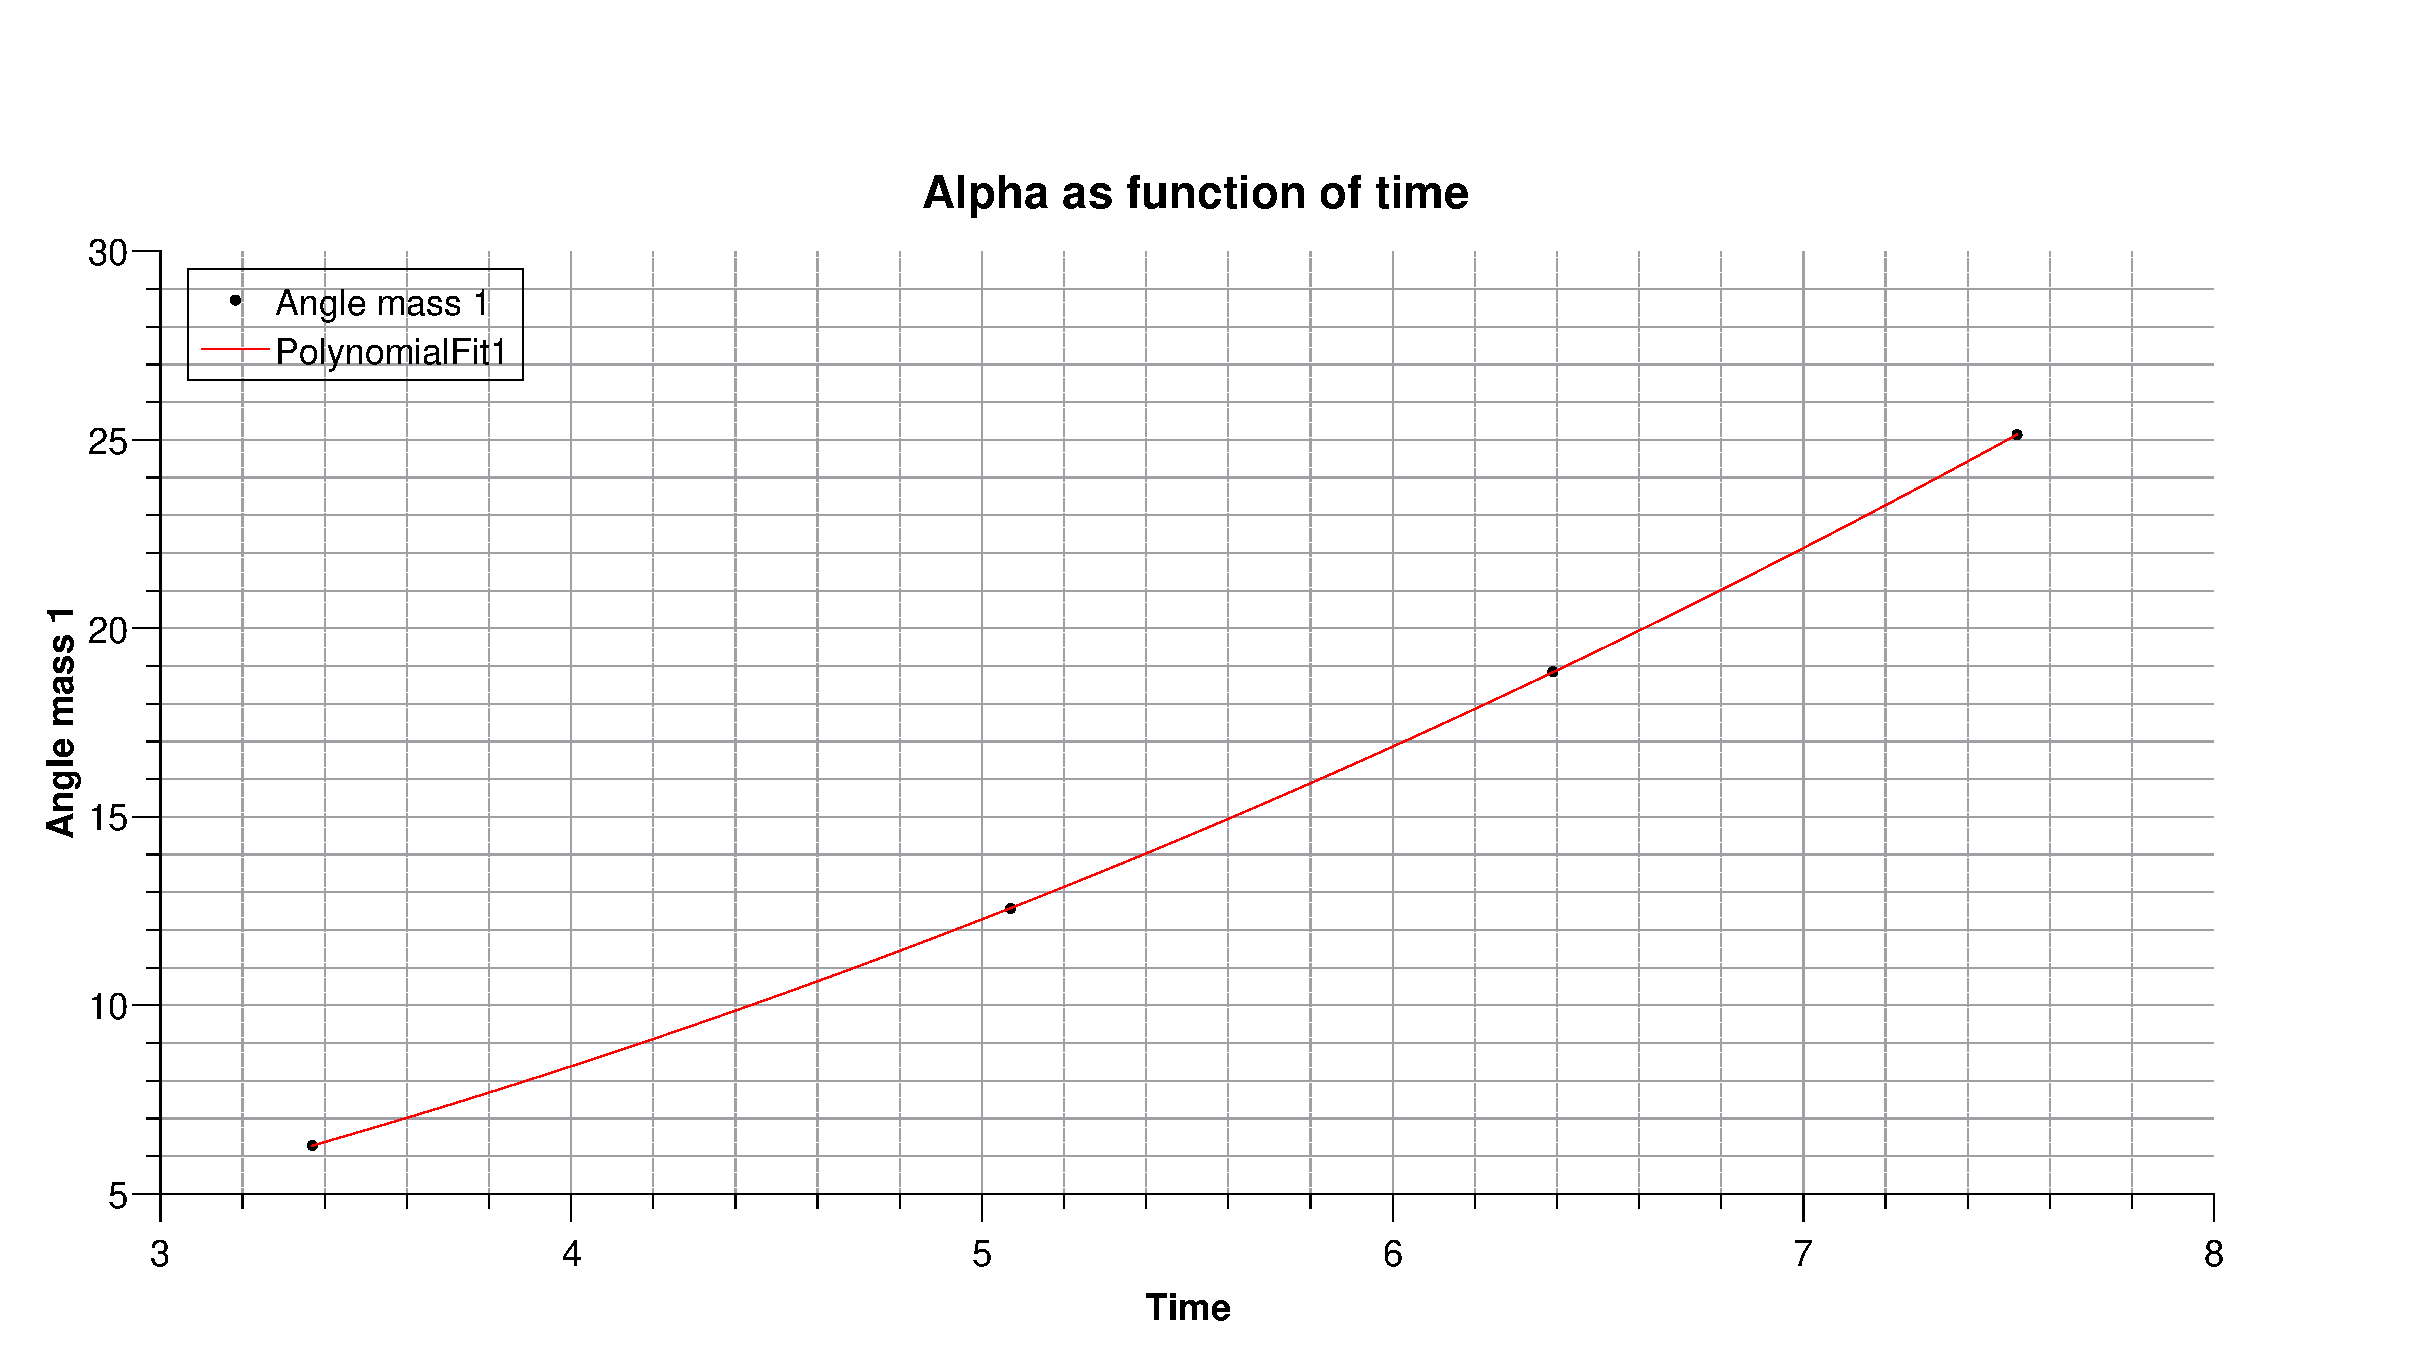
\includegraphics[width=11cm]{mass1_AlphaFunctionOfTime.eps}
        \caption{Alpha as function of time for mass 1}
        \label{fig:my_label}
    \end{figure}

    \begin{figure}[h]
        \centering
        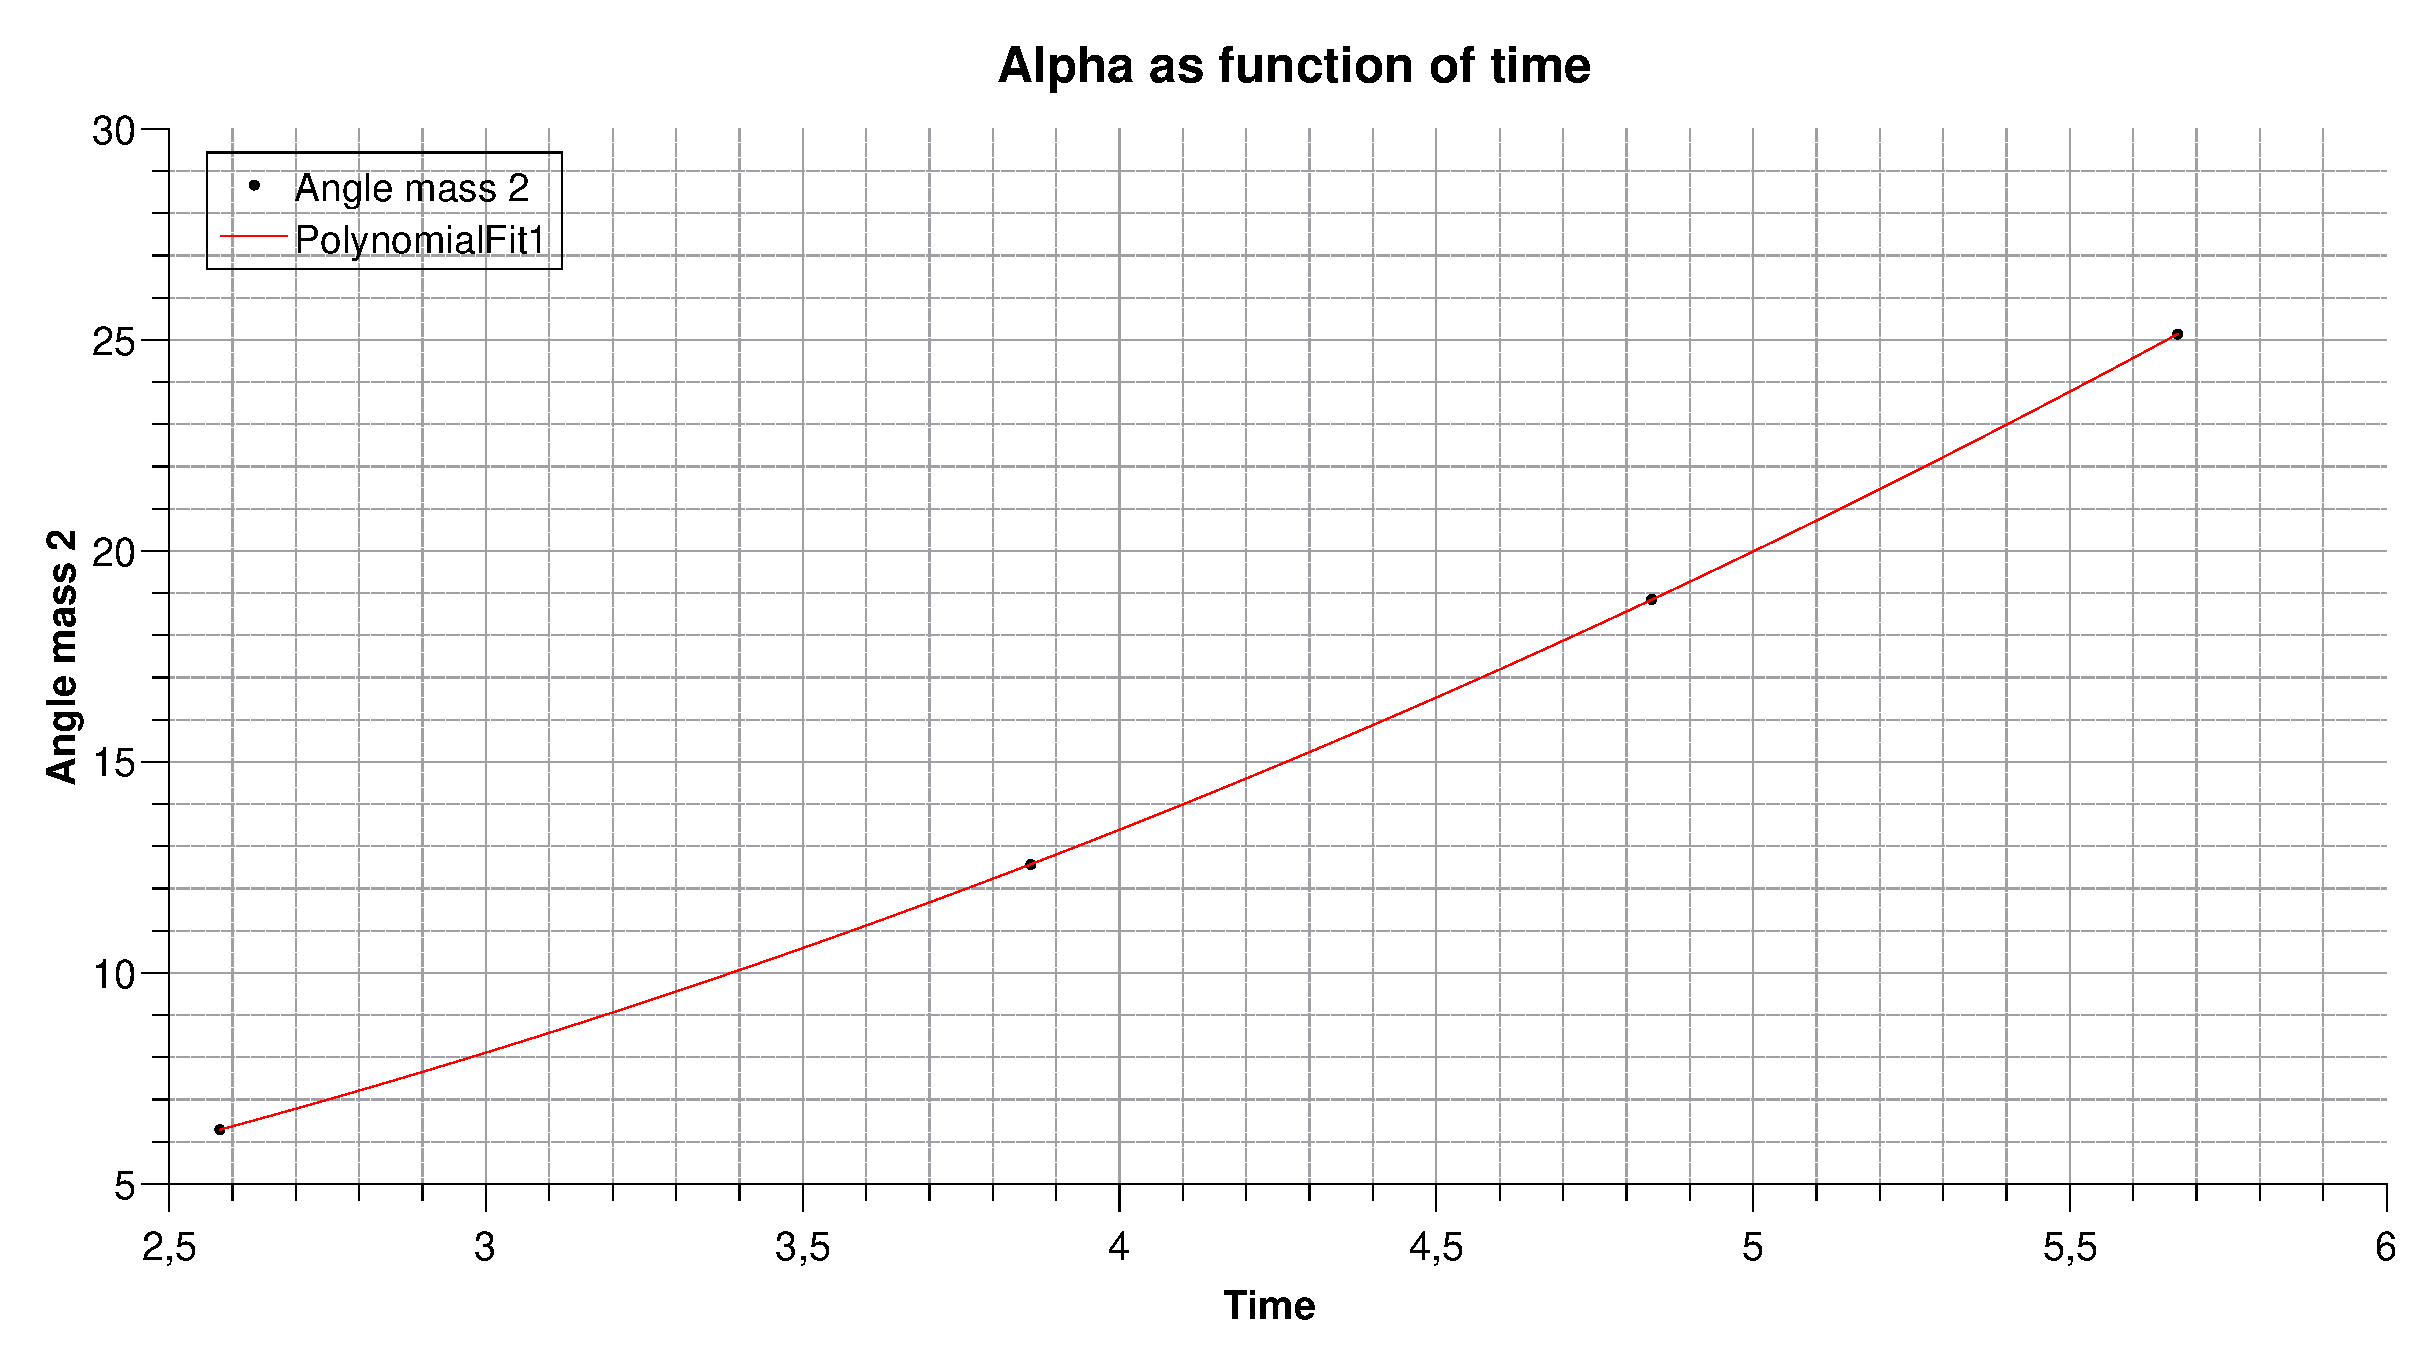
\includegraphics[width=11cm]{mass2_AlphaFunctionOfTime.eps}
        \caption{Alpha as function of time for mass 2}
        \label{fig:my_label}
    \end{figure}
    
    \begin{figure}[h]
        \centering
        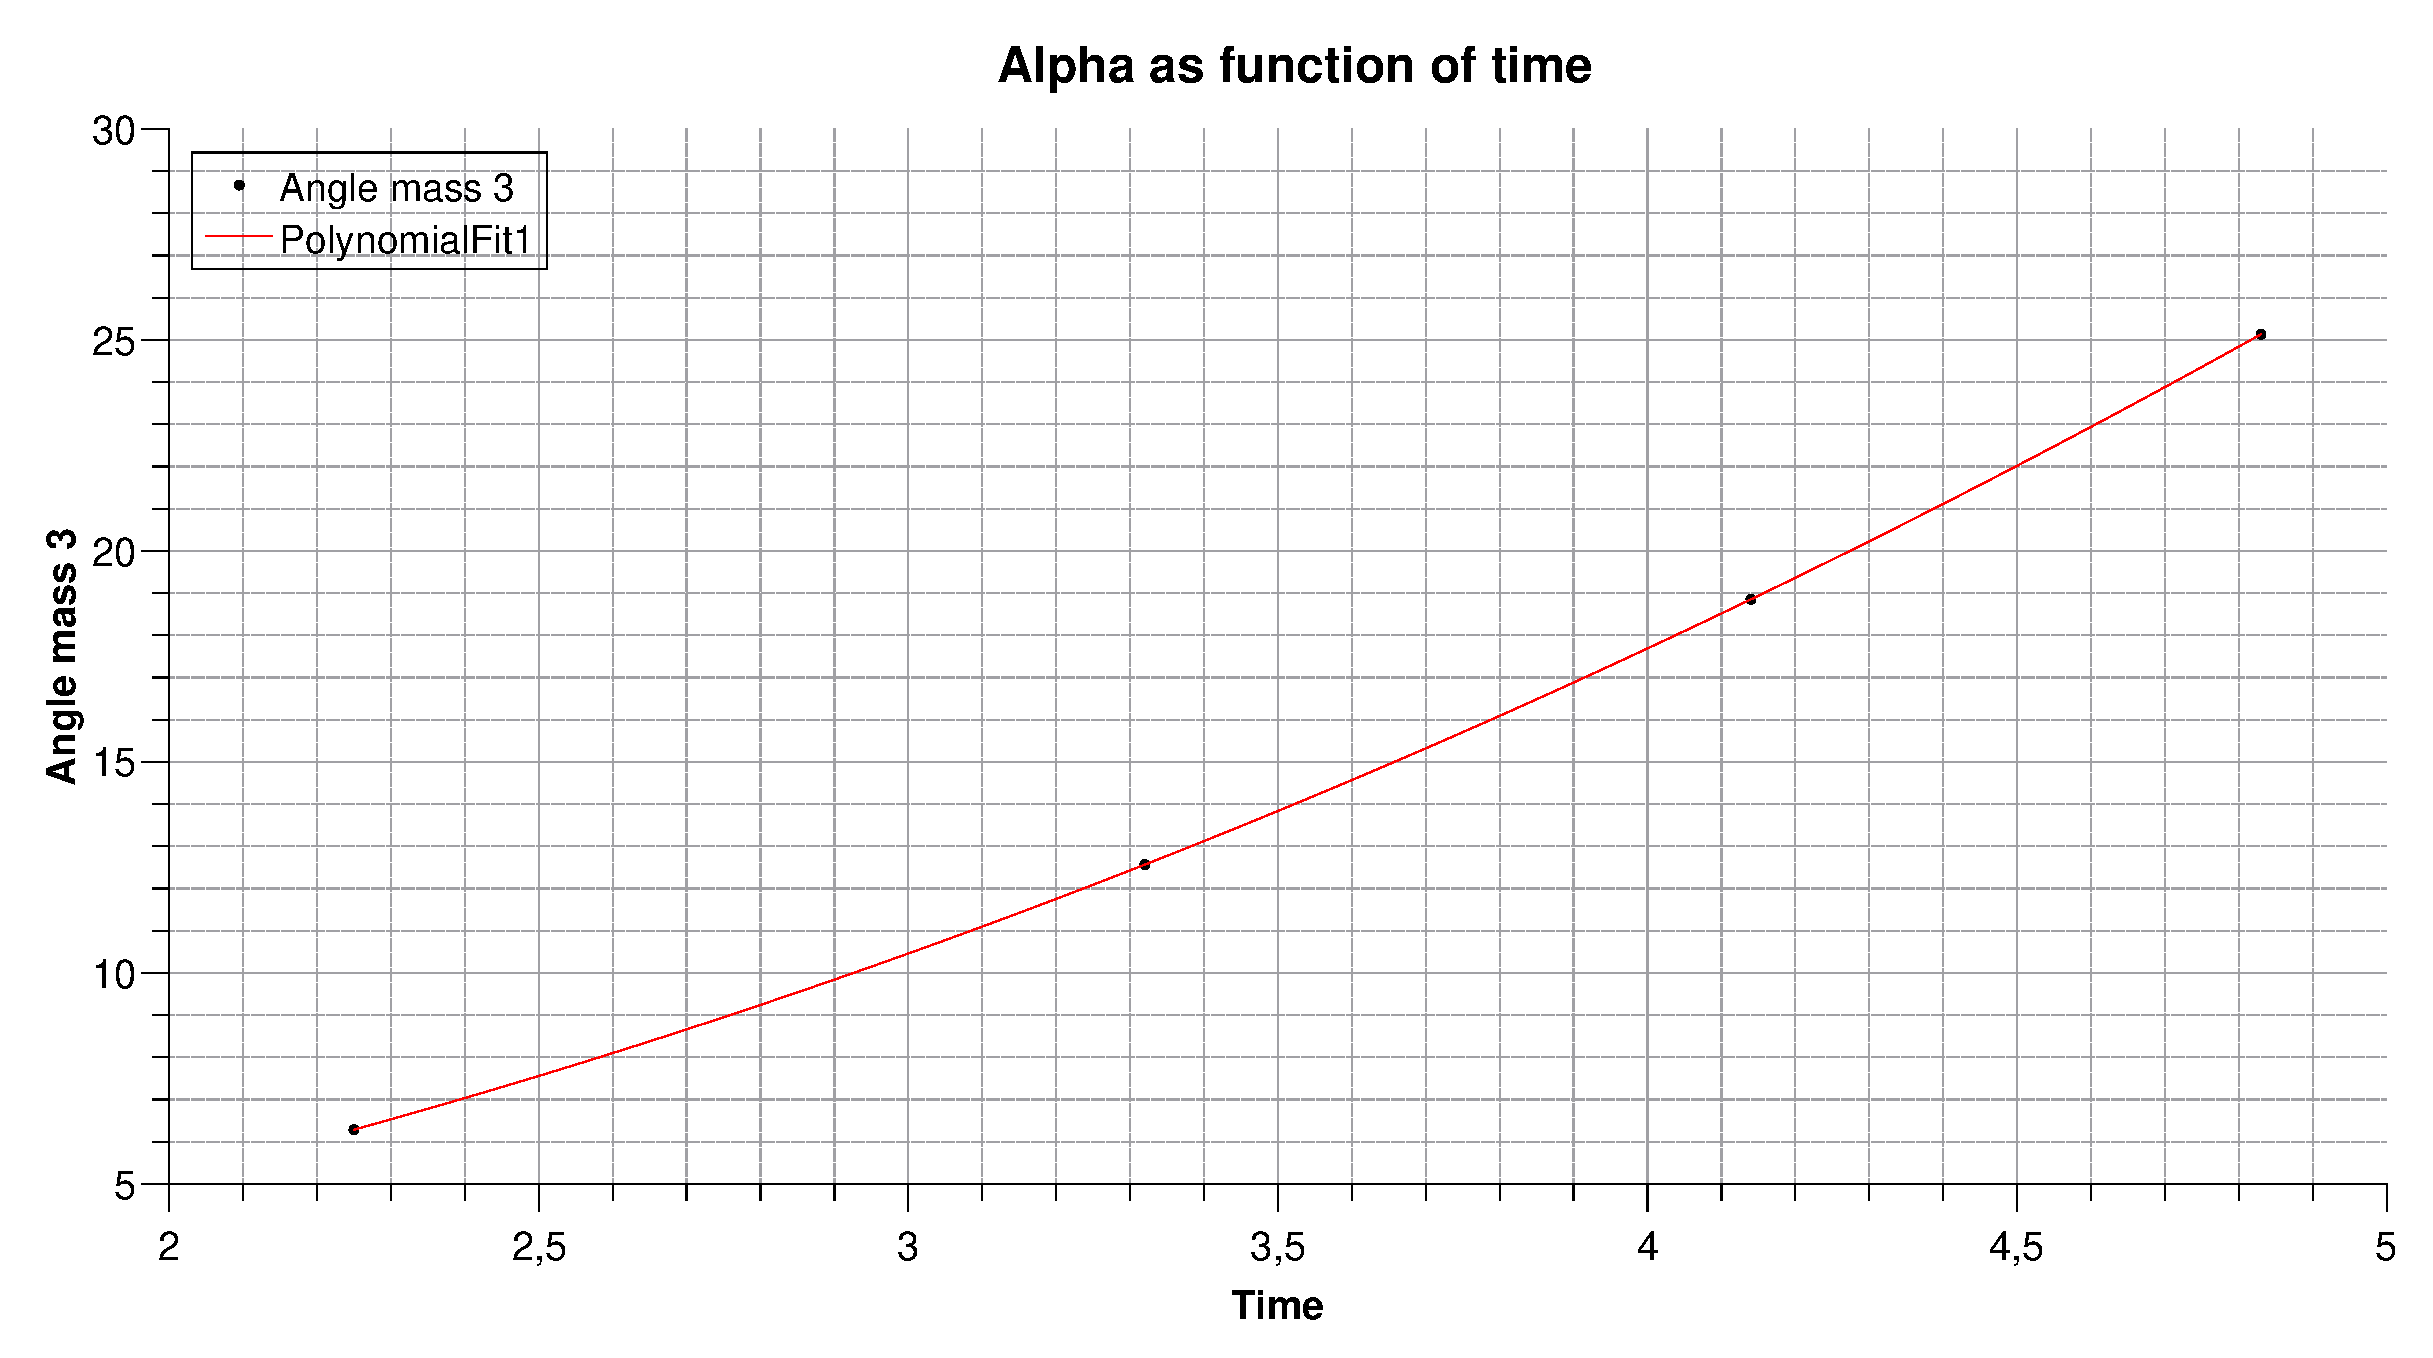
\includegraphics[width=11cm]{mass3_AlphaFunctionOfTime.eps}
        \caption{Alpha as function of time for mass 3}
        \label{fig:my_label}
    \end{figure}
    
    \begin{figure}[h]
        \centering
        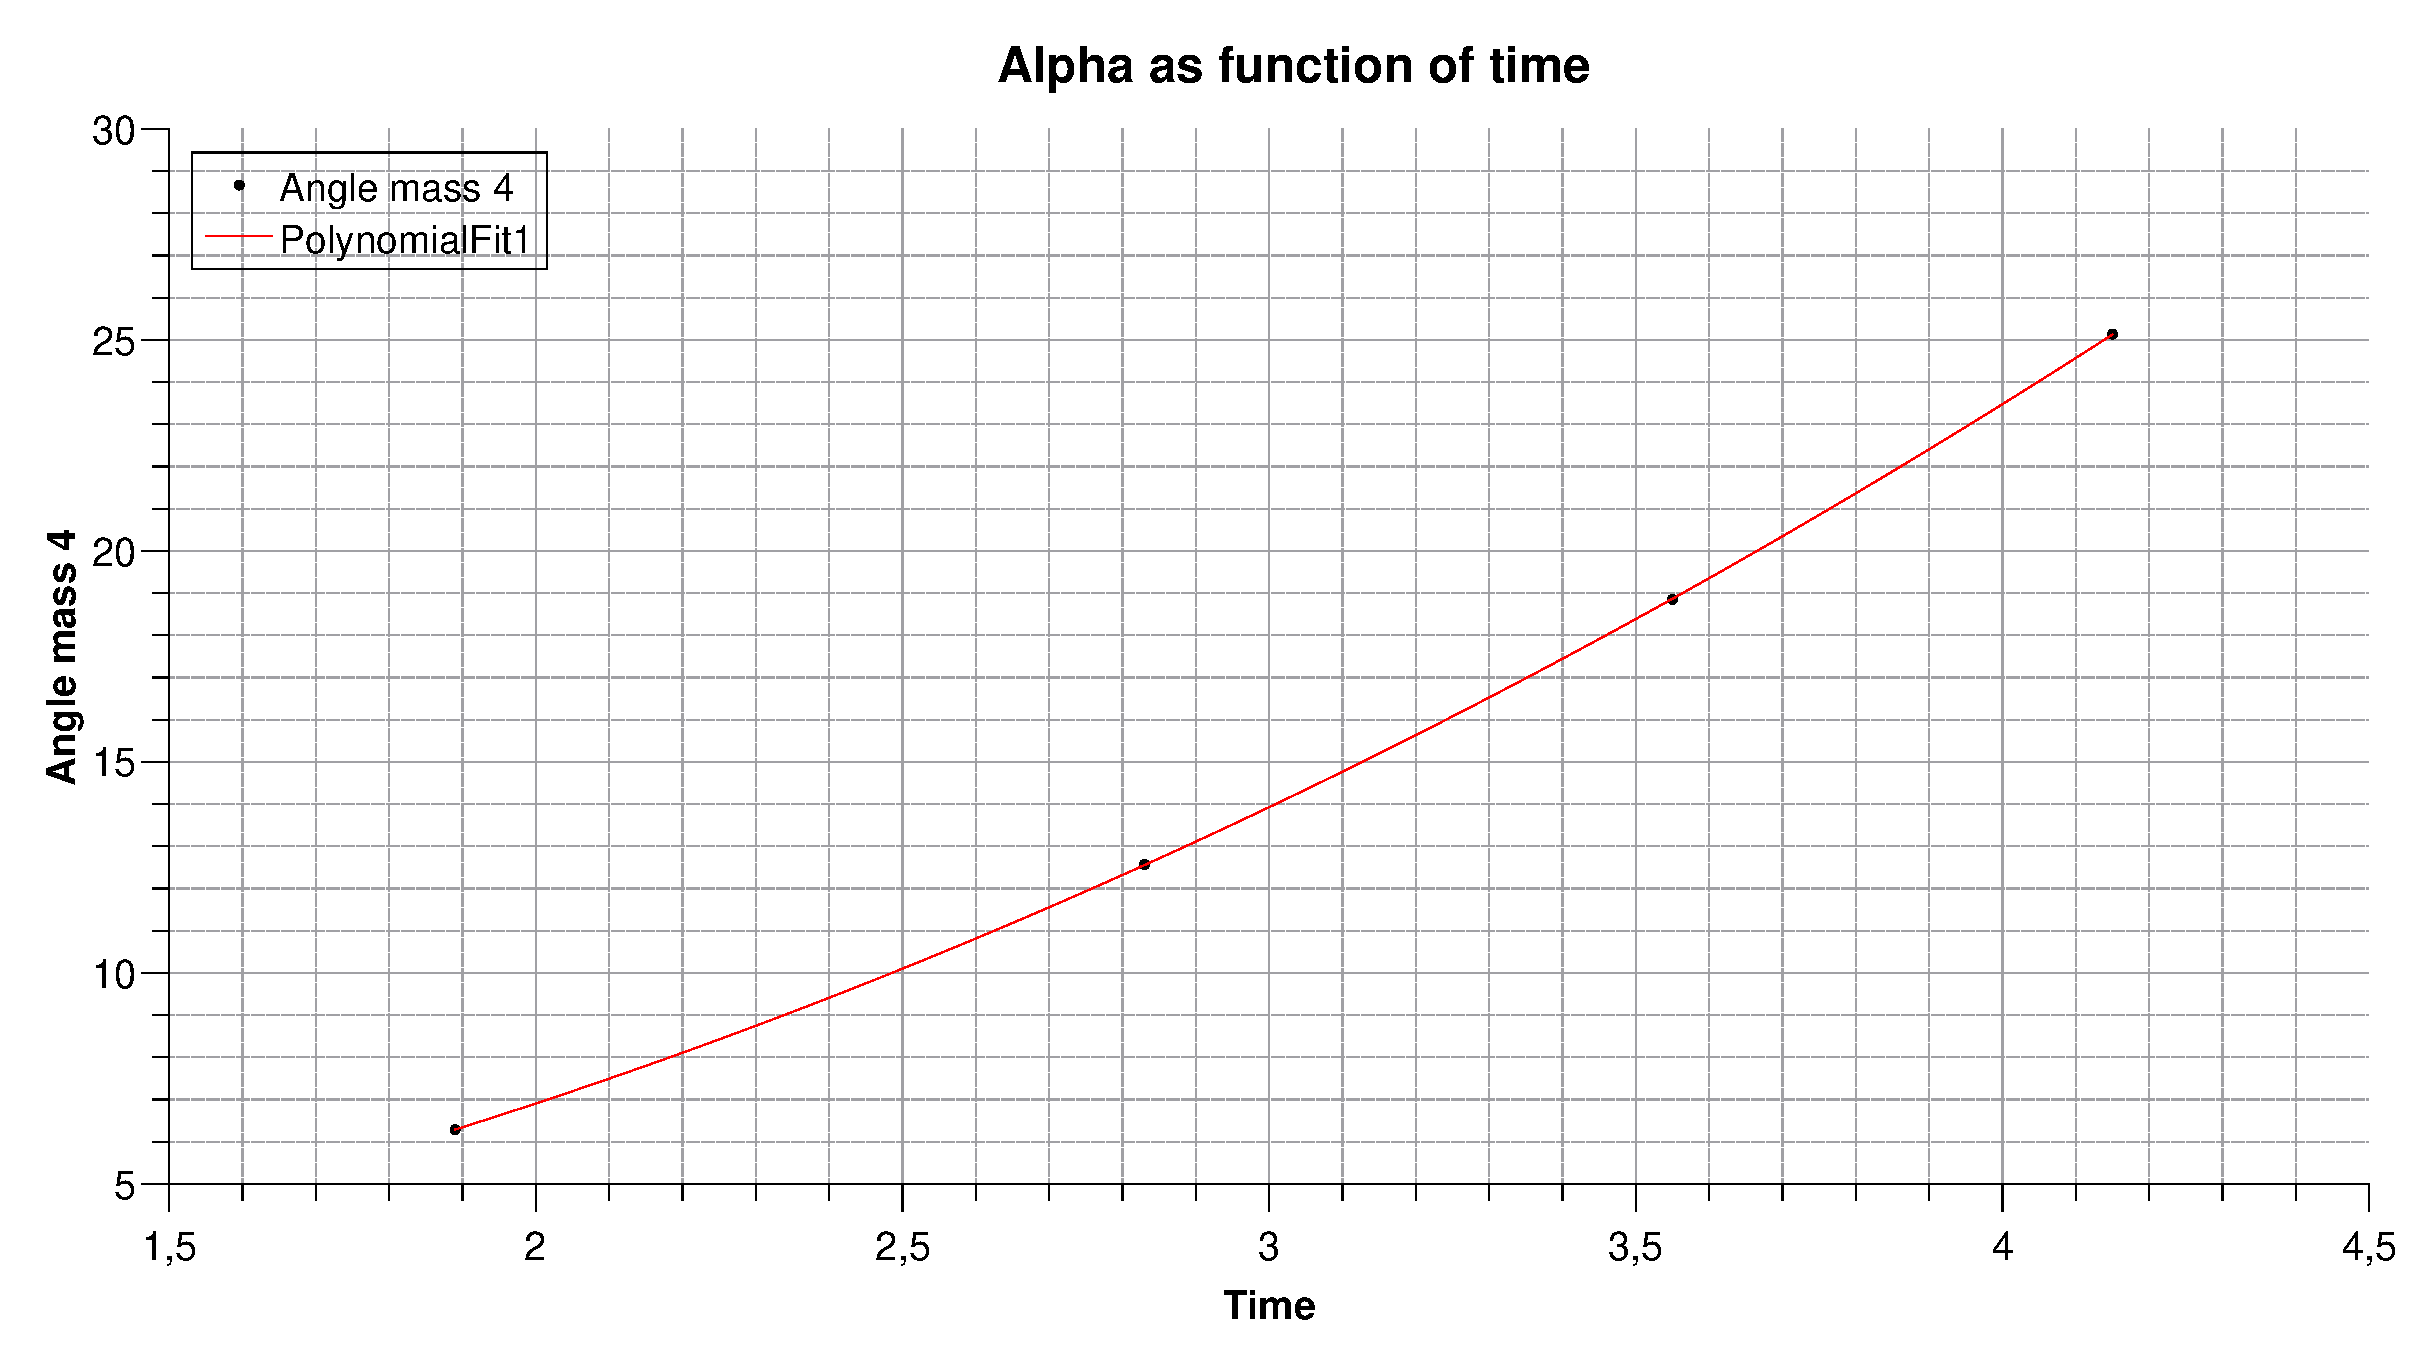
\includegraphics[width=11cm]{mass4_AlphaFunctionOfTime.eps}
        \caption{Alpha as function of time for mass 4}
        \label{fig:my_label}
    \end{figure}
    
    \begin{figure}[h]
        \centering
        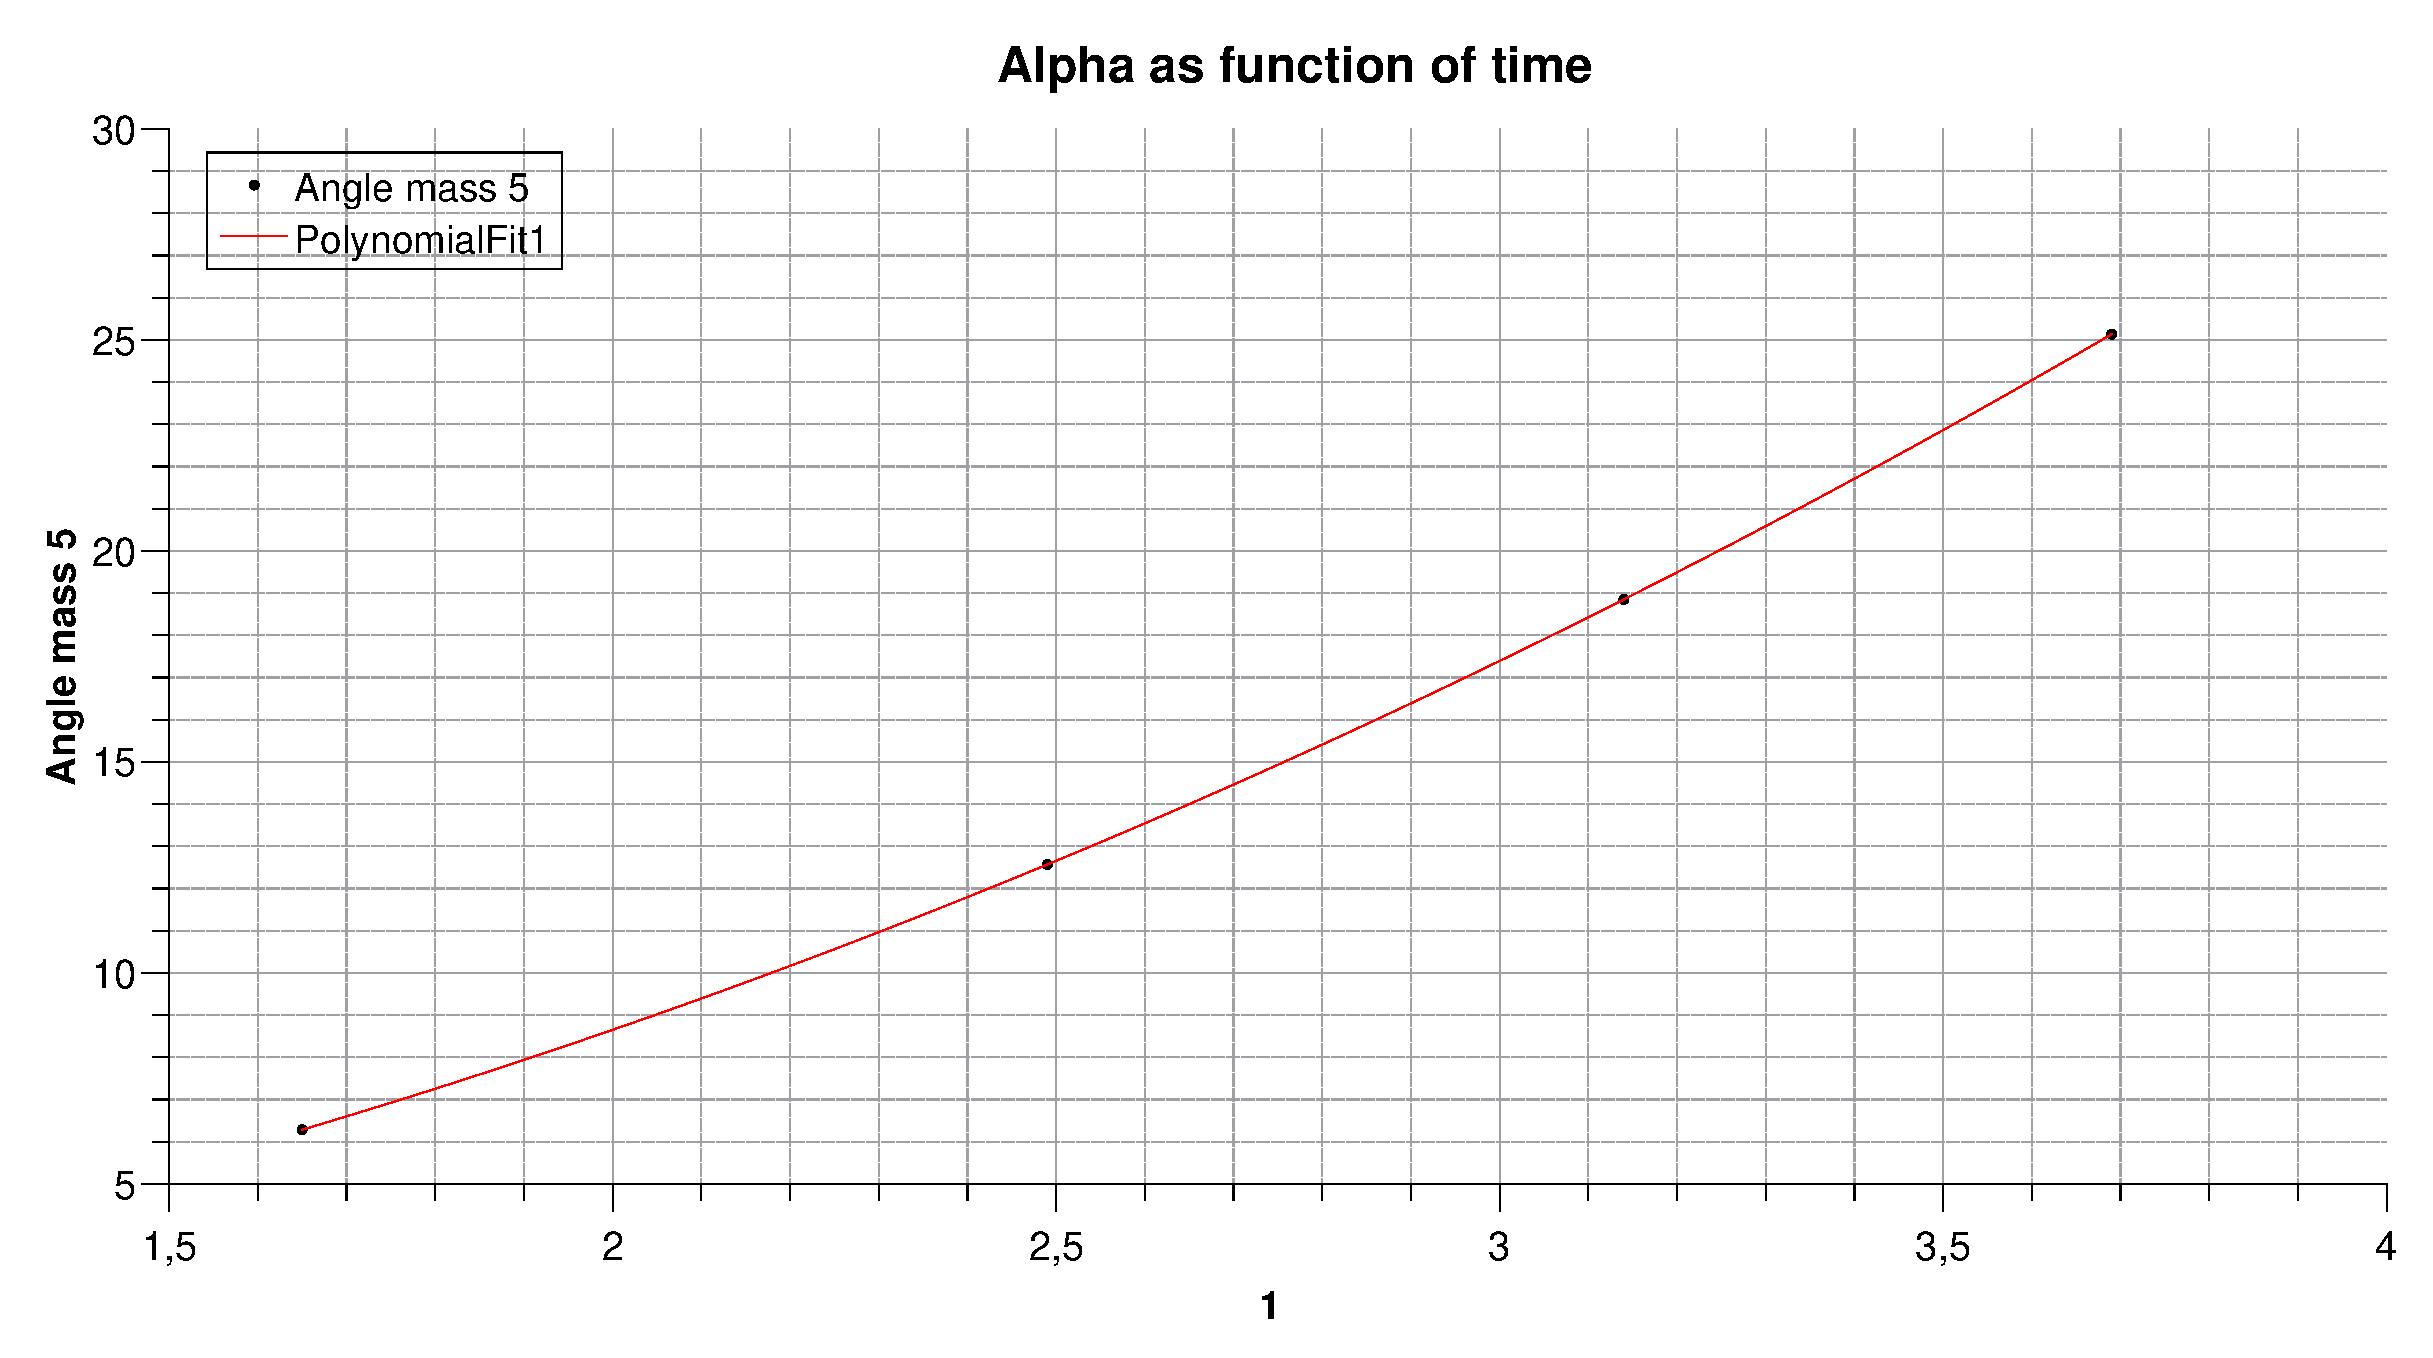
\includegraphics[width=11cm]{mass5_AlphaFunctionOfTime.eps}
        \caption{Alpha as function of time for mass 5}
        \label{fig:my_label}
    \end{figure}
\end{document}